\documentclass[10pt,a4paper]{article}
\usepackage[utf8]{inputenc}
\usepackage{amsmath}
\usepackage{amsfonts}
\usepackage{amssymb}
\usepackage{geometry}
\usepackage{verbatim}
\usepackage{enumerate}
\usepackage{fancyvrb}
\usepackage{graphicx}
\usepackage{hyperref}
\usepackage{tikz}
\usetikzlibrary{positioning}
\usetikzlibrary{shapes,snakes}
\usepackage[english]{babel}

\geometry{legalpaper, margin=1.5in}

\author{William Schultz}
\begin{document}
\title{Strongly Connected Components}
\author{William Schultz}
\maketitle

In a \textit{directed graph} $G=(V,E)$, we say that two nodes, $u$ and $v$, are \textit{connected} if there is a path from $u$ to $v$ and a path from $v$ to $u$. This relation is reflexive, symmetric, and transitive, so it is an equivalence relation on nodes. Thus, it partitions $V$ into disjoint sets, which are called the \textit{strongly connected components} of the graph. That is, a strongly connected component is a subset of nodes in $V$ such that every node in the component can reach every other node in the component.

If we shrink down each strongly connected component into a single node, and draw an edge between two of them if there is an edge from some node in the first to some node in the second, the resulting graph has to be a \textit{directed acyclic graph (dag)}. That is, it has no cycles. This holds since if there was a cycle containing several strongly connected components, then this would merge them all into a single strongly connected component. In other words, \textit{every directed graph is a dag of its strongly connected components.} \href{https://en.wikipedia.org/wiki/Tarjan%27s_strongly_connected_components_algorithm}{Tarjan's algorithm} can be used to compute the strongly connected components of a directed graph in time linear in the number of nodes and edges i.e. in $O(|V| + |E|)$.

\begin{center}
    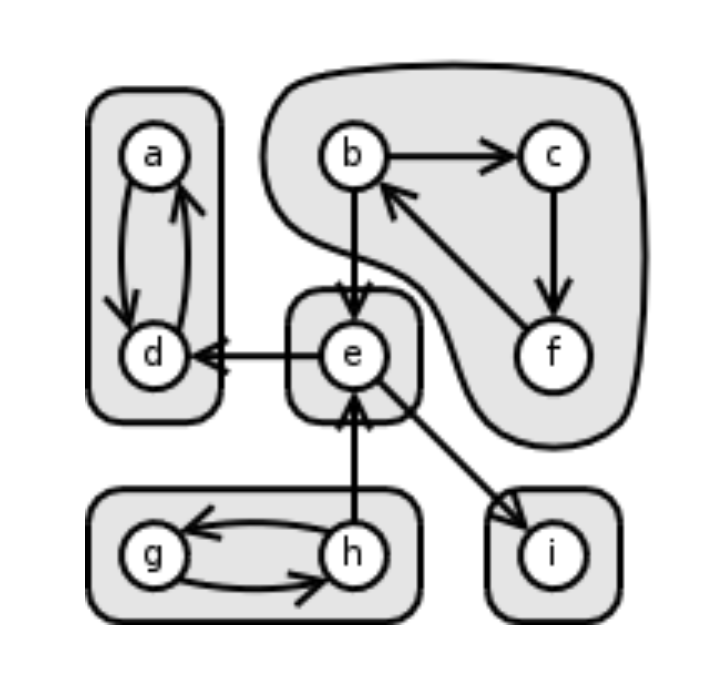
\includegraphics[scale=0.3]{sccs.png}
\end{center}

% \bibliographystyle{plain}
% \bibliography{../references.bib}

\end{document}